% \part{Related Works and Preliminaries}

\section {Related Work}

\subsection {Motion Parallax}

Motion parallax is a visual illusion that occurs when objects at different distances move across the observer's field of view. This phenomenon is a key depth cue in human vision, enabling the perception of depth and distance in the absence of stereoscopic vision. Principles of motion parallax can provide depth information to human brain's neural is the comparation of motion speed of different objects in the same view. e.g., when a person moves his head, objects closer to the observer appear to move faster than objects further away, providing a sense of depth and distance. Hanes et al.(2008) explain the mathemetical details of motion parallax, providing geometry and experimental evidence of it\cite{Hanes2008}, shown as Fig.3.

\begin{figure}[htb]
    \centering
    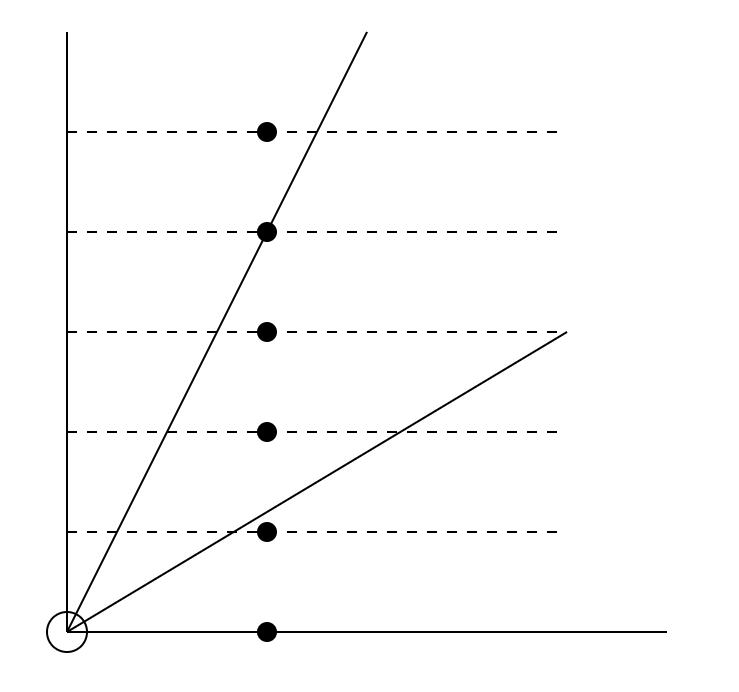
\includegraphics[width=0.5\textwidth]{figures/Introduction/motion.png}
    \caption{Motion parralax reminder: view angle difference is a good cue for motion derectory, while object's movement distance is velocity's\cite{Hanes2008}}\label{F:test-a}
\end{figure}

This effect is widely used in 3D display systems: Lee et al. (2019) designed a head-traking system based on Nintendo Wii remote, constructed a depth illusion with the application of motion parallax\cite{Lee}. Apple's IOS7 also introduced a light motion parallax effect. By move applications' icons lightly when users move their phone, Apple provides a more immersive and interactive experience for users.\cite{Apple2014}.
\subsection{Face  Landmark Detection}
From early techniques, face landmark is mainly implemented by statistical and simple machine learning methods. The \textbf{Active Shape Model (ASM)}, \textbf{Active Appearance Model (AAM)}, and \textbf{Constrained Local Model (CLM)} \cite{WANG201850} \cite{Khabarlak_2022} are foundational methods that employ statistical models to fit a deformable face mesh, optimized for controlled environments but underperforming in in-the-wild scenarios. Subsequent advancements, such as \textbf{Ensemble of Regression Trees (ERT)} \cite{Kazemi_2014_CVPR} employed by \textbf{dlib}, improved accuracy by using a cascade based on gradient boosting\cite{saberian2014boosting}, making it highly efficient for real-time applications despite its limitations with pose variations.

\begin{figure}[htb]
    \centering
    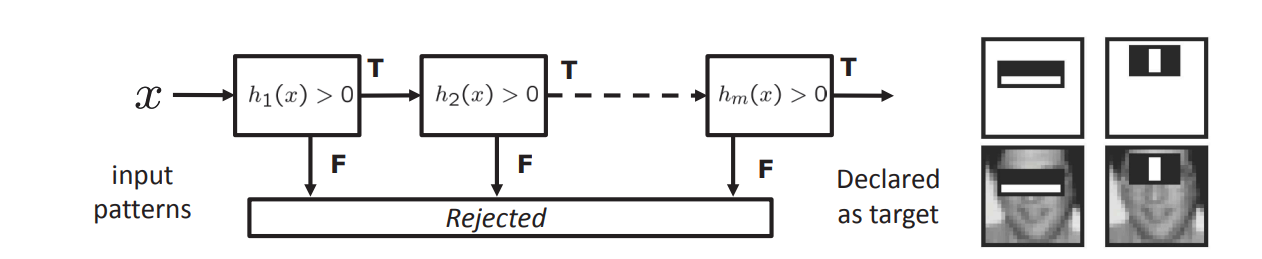
\includegraphics[width=1\textwidth]{figures/Introduction/cascade.png}
    \caption{Cascade based gradient boosting }\label{F:test-a}
\end{figure}

The evolution towards neural network-based approaches has introduced a diverse array of backbones, enhancing the detection capabilities under unconstrained conditions. Techniques such as the \textbf{Hourglass} \cite{Newell_2016_ECCV} and \textbf{HRNet} \cite{Sun_2019_CVPR} architectures leverage heatmap-based methods to improve landmark localization accuracy by predicting probabilistic heatmaps for each landmark . These methods are robust against pose variations and occlusions, crucial for applications requiring high fidelity in dynamic environments.
\textbf{Style Aggregated Network (SAN)}\cite{Dong_2018_CVPR} employs ResNet-152 \cite{He_2016_CVPR} to handle variability in image styles by stabilizing landmark detection across different photographic conditions, illustrating the importance of adaptive models in diverse real-world applications.

YOLO-series\cite{Redmon_2016_CVPR} are also considered as a efficient method in face landmark detection. As a one-stage object detection model, YOLO detect objects' position and classes by directly inference features extract by CNN model. Base on YOLO, Qi et al. (2022) developed \textbf{YOLO5Face}\cite{Qi2022YOLO5Face}, a face detector built upon the YOLOv5 object detection framework. The model incorporates modifications such as a landmark regression head and various optimizations for processing both large and small faces effectively. YOLO5Face is designed to provide robust face detection capabilities across different model sizes, catering to various application requirements from high-performance setups to real-time detection on mobile or embedded devices. The detector achieves state-of-the-art performance on the WiderFace dataset, demonstrating its efficiency and accuracy in diverse conditions. In following two years, YOLOv7-face\cite{YOLOv7Face} and YOLOv8-face\cite{YOLOv8Face} is developed, which further improve the performance of face detection and landmark detection.

% \begin{figure}[htb]
%     \centering
%     \includegraphics[width=0.6\textwidth]{example-image-a}
%     \caption{YOLOv1 structure}\label{F:test-a}
% \end{figure}

In 2023, Wu et developed \textbf{YuNet}\cite{Wu_2023}, an advanced face detection model specifically engineered for edge computing devices, which emphasizes minimal model size and maximized computational efficiency. The architecture of YuNet incorporates a streamlined feature extraction backbone and a simplified pyramid feature fusion technique, tailored to meet the stringent performance requirements of mobile and embedded systems with limited processing capabilities. This model is distinguished by its ability to deliver high-speed performance with an exceptionally low parameter count, making it particularly well-suited for real-time applications where both speed and accuracy are critical, yet resources are constrained.


\subsection{Target Tracking}
During these decades, target traking problem has gains lots of attetion in academic and industrial firld due to the universality of application. With sensor information stream input, tracking algorithms estimate target's motion state, applicated them in next-timestamp's pose estimation. Target tracking algorithms can mainly be divided into three categories: \textbf{Batch Processing}, \textbf{Recursive} and \textbf{Optimization-Based}\cite{KumarMondal2021}. Batch Processing methods observe one time period operate one specific time period to estimate target's motion state, with common algorithms like MLE, PLS, GA and sequencial networks. A typical problem of Batch Processing latency issue and data requirement, since batch processing need to wait for all data to be collected before processing.\cite{KumarMondal2021}. 

\begin{figure}[htb]
    \centering
    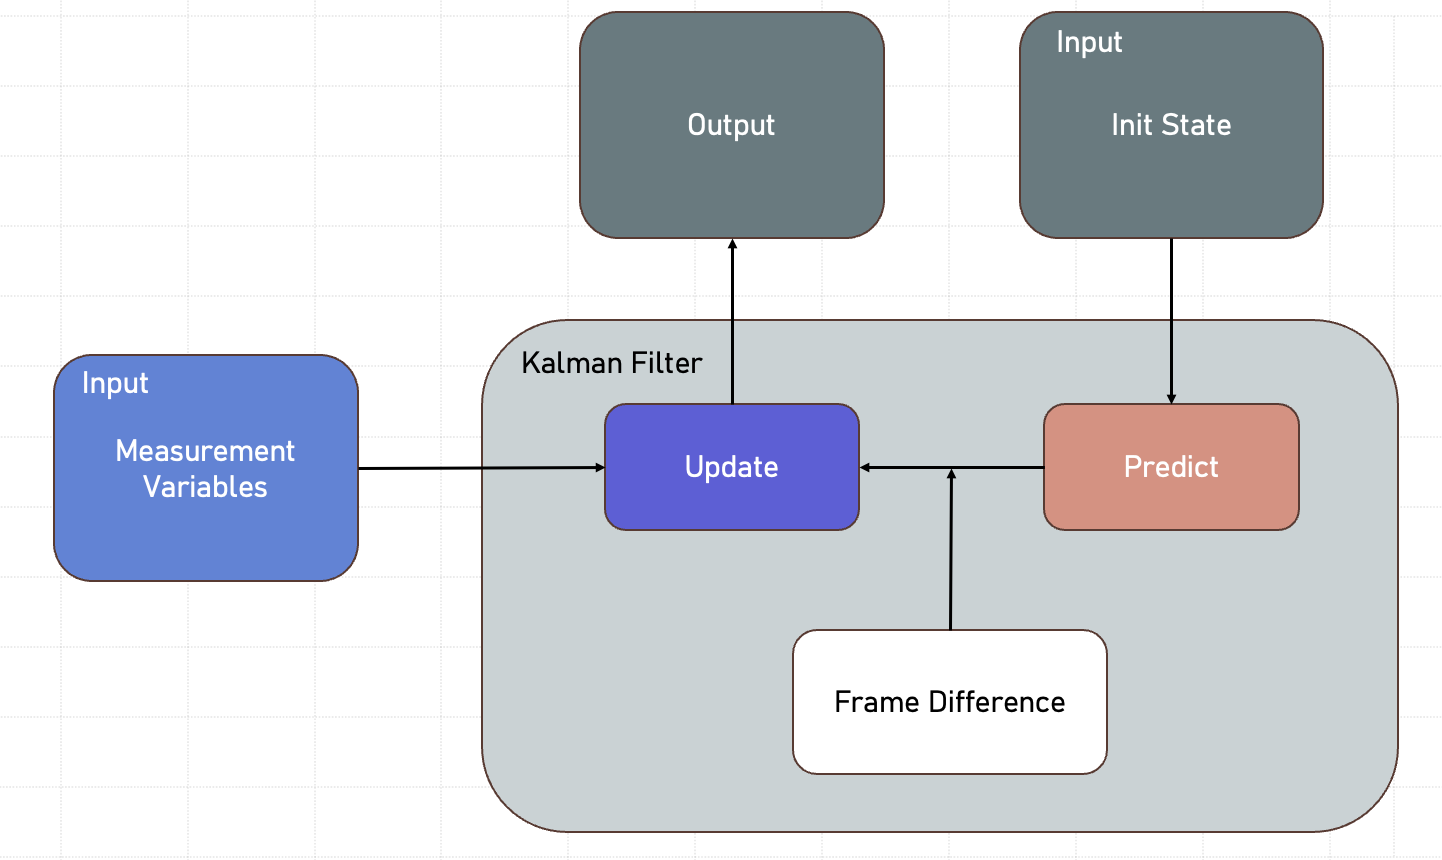
\includegraphics[width=1\textwidth]{figures/Introduction/KalmanFilter.png}
    \caption{Kalman filter working flow}\label{F:test-a}
\end{figure}

Recursive-based methods, typically Sequential Bayesian filter, performance better in real-time tracking and unbiased estimates\cite{KumarMondal2021}. One powerfule variant of Sequential Bayesian filter is Kalman Filter, proposed by Rudolf E. Kálmán in 1960\cite{Kalman1960}, designed to estimate target's motion state with noisy sensor information. Kalman Filter is widely used in target tracking, pose estimation, and sensor fusion.


Another category of target tracking is Optimization-Based methods, developed on the basis of loss functions of tracking methods.\cite{KumarMondal2021}. Optimization-Based methods are more flexible and can be applied in various tracking scenarios, with common algorithms like Particle Filter, Mean Shift, and Deep Learning-based methods. However, since loss-fucntions' optimization introduce extra complexity, Optimization-Based methods are usually more computational expensive than Recursive-based methods.

\nocite{Khabarlak_2022}

\section {Preliminaries}
This section introduces the basic concepts and technologies used in this project, including face landmark detection, Perspective-N-Point (PnP) problem, Kalman Filter, Perspective Projection and Off-axis Perspective Projection. We will introduce YuNet in section 3.1, and review the PnP problem in section 3.2. In section 3.3, we will introduce the Kalman Filter, including a simple derivation. In section 3.4, we will introduce the perspective projection and off-axis perspective projection, and explain why off-axis perspective projection is needed in our research.
\subsection{Face Landmark Detection}
Face landmark detection is one of the main tasks in computer vision. It is used to detect the key points of a face, such as the eyes, nose, and mouth. These key points can be used for various applications, such as face recognition, emotion detection, and head pose estimation. There are many different methods for face landmark detection, including traditional computer vision techniques and deep learning-based approaches. In this project, we will use a deep learning-based approach for face landmark detection, as YuNet provided in Sec2.2. OpenCV 4.5.4\cite{opencv_4_5_4} introduced YuNet in 2021 as one of face landmark detection API, which provide a fast and convinience way to complete face landmark detection task. In addition, a research compare YuNet a with traditional haar cascade detection in dlib, and YuNet performs better in both performance and accuracy. \cite{chen2022opencv}.

\subsection{Perspective-N-Point (PnP) Problem}
Perspective-N-Point (PnP) problem is a fundamental problem in computer vision, which is used to estimate the pose of a camera given a set of 3D points and their corresponding 2D projections. The PnP problem is commonly used in applications such as augmented reality, camera calibration, and robot localization. There are many different algorithms for solving the PnP problem, including the Direct Linear Transform (DLT) method, the Levenberg-Marquardt algorithm, and the RANSAC algorithm. 

\begin{figure}[htb]
    \centering
    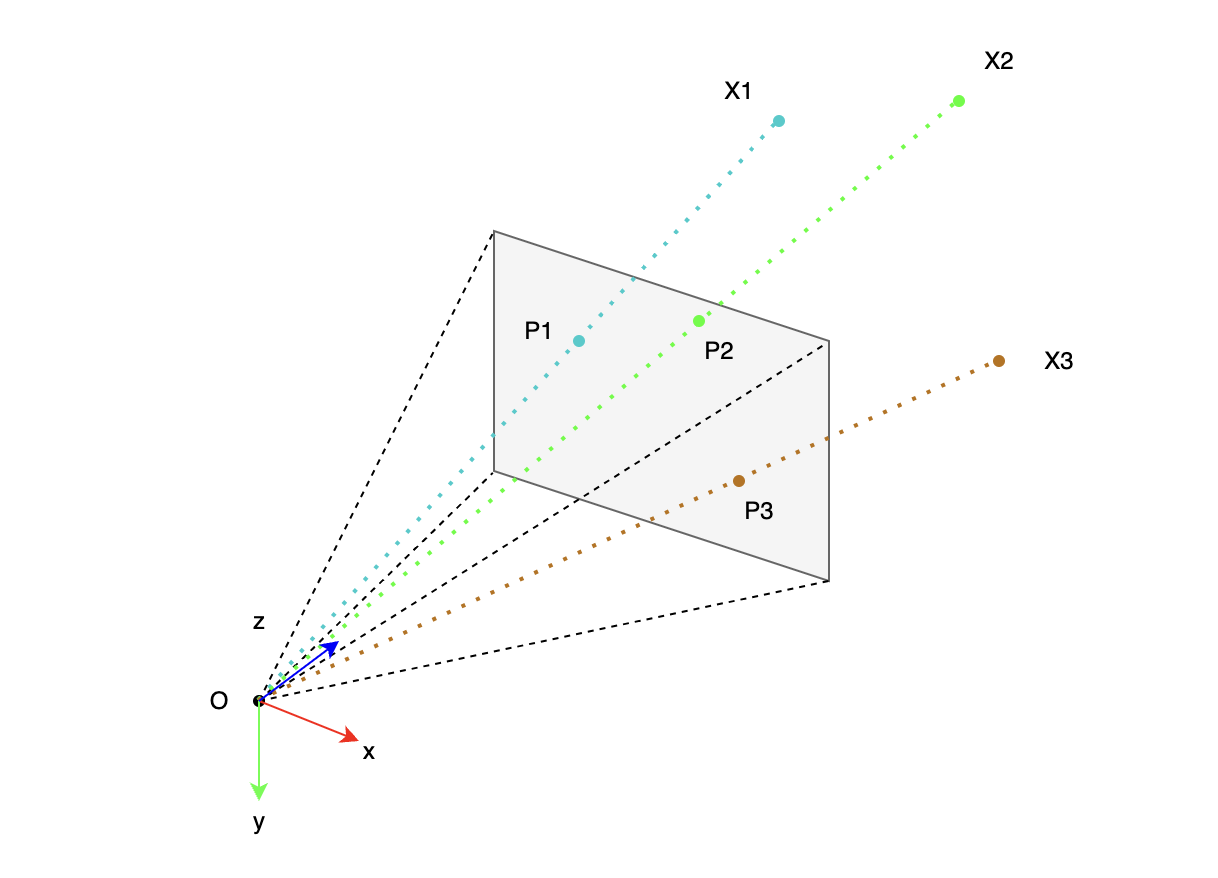
\includegraphics[width=1\textwidth]{figures/Introduction/PnP.png}
    \caption{Perspective-N-Point(PnP) problem}\label{F:test-a}
\end{figure}


\subsection{Kalman Filter}
Using face position provided by pnp solver directly usually is an effeient way, but not stable enough to cover noises from possible environments.  Since keypoints provided by detector is not stable enough to get a steady result, position solve by pnp-solver often meet unexpected oscillation and jittering. To solve the problem, we introduce kalman filter as a filter to smooth the movement of human head. 

Kalman Filter is a specific type of recursive Bayesian filter, which is used to estimate the state of a linear dynamic system from a series of noisy measurements. As a varietas of Bayesian filter, Kalman filter combain the prior knowledge of the system with the current measurement to provide an optimal estimate of the state of the system by a self-adjusting kalman gain $K$. 

The Kalman Filter is based on a linear dynamical system model, based on following elements:
\begin{itemize}
    \item State Vector $x_k$: State to be estimated of the  system.
    \item Measurement Vector $z_k$: Variable can be measured by sensors of the system. Note the measurement is noisy.
    \item State Transition Matrix $F_k$: State transition matrix, which describe the state transition of the system from prior state to current state.
    \item Measurement Matrix $H_k$: Measurement matrix, which describe the mapping from state space to measurement space.
    \item Process Noise Covariance Matrix $Q_k$: Covariance matrix of the process noise.
    \item Measurement Noise Covariance Matrix $R_k$: Covariance matrix of the measurement noise.
    \item Kalman Gain $K_k$: Gain of the Kalman filter, which is used to adjust the weight of the prior state and the measurement.
    \item State Covariance Matrix $P_k$: Covariance matrix of the prior state.
\end{itemize}

The Kalman Filter consists of two main steps: the prediction step and the update step. In the prediction step, filter predict the state of the system based on the prior state and the state transition matrix and update prior state covariance P:
\begin{equation}
    \hat{x}_{k|k-1} = F_k \hat{x}_{k-1|k-1} 
\end{equation}
\begin{equation}
    P_{k|k-1} = F_k P_{k-1|k-1} F_k^T + Q_k
\end{equation}


Once the measurement is available, the filter update the state of the system based on the measurement and the measurement matrix:
\begin{equation}
        K_k = P_{k|k-1} H_k^T (H_k P_{k|k-1} H_k^T + R_k)^{-1}
\end{equation}
\begin{equation}
        \hat{x}_{k|k} = \hat{x}_{k|k-1} + K_k(z_k - H_k \hat{x}_{k|k-1})
\end{equation}
\begin{equation}
        P_{k|k} = (I - K_k H_k) P_{k|k-1} 
\end{equation}

In update step, kalman gain is updated based on the measurement and the prior state covariance, and providing the optimal estimate of the state of the system in next step.

\subsection{Perspective Projection and Off-axis Perspective Projection}

Perspective projection is a common projection method in computer graphics and daily life. It is used to project a 3D point onto a 2D plane. Consider a 3d object point, perspective projection generated 2d coordinate by mapping it to a 2 * 2 * 2 rectangular-projection cube, where $x$ and $y$ are the 2D position and $z$ is the depth information of the 3D point.

As camera field of view($fov$) given, we can generate the perspective projection matrix as:

\[
\begin{bmatrix}
\frac{\cot \left( \frac{\text{fovy}}{2} \right)} {aspect} & 0 & 0 & 0 \\
0 & \cot \left( \frac{\text{fovy}}{2} \right) & 0 & 0 \\
0 & 0 & -\frac{f+n}{f-n} & -\frac{2fn}{f-n} \\
0 & 0 & -1 & 0
\end{bmatrix}
\]
Where $f$ is the far plane, $n$ is the near plane, and $aspect$ is the aspect ratio of the view plane. Fully explanation of perspective projection can be found in \cite{ahn_opengl_projection_matrix}.
    
\begin{figure}[htb]
    \centering
    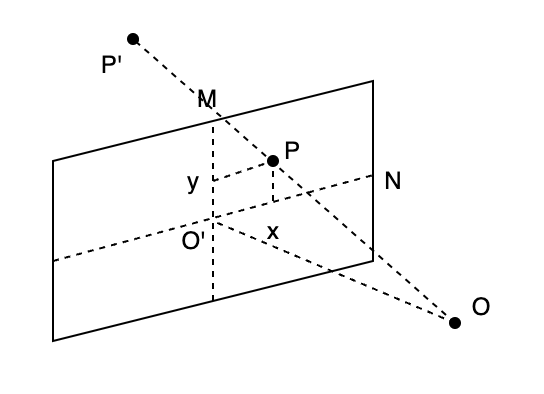
\includegraphics[width=0.7\textwidth]{figures/Preliminaries/pinCamera.png}
    \caption{Pinhole camera model, where $O$ is observer's position, $O'$ is view point, $O'MN $ is view plane, $P$ is the 2D projection on view plane of a 3D point, and $M$, $N$ is the orthogonal projection from the viewpoint to the upper/right boundary of the plane.}\label{F:test-a}
\end{figure}

% \begin{figure}[htb]
%     \centering
%     \begin{subfigure}[t]{.45\linewidth}
%         \centering
%         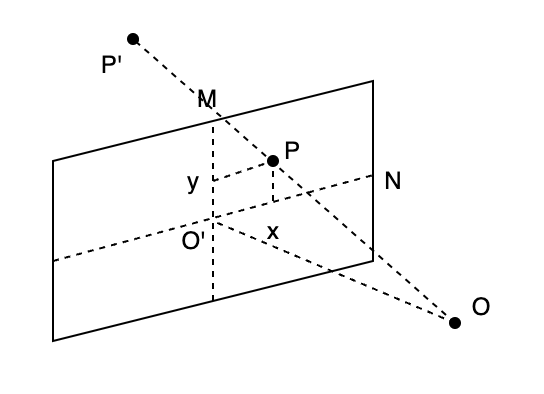
\includegraphics[width=1\textwidth]{figures/Preliminaries/pinCamera.png}
%         \caption{Pinhole camera model, where $O$ is observer's position, $O'$ is view point, $O'MN $ is view plane, $P$ is the 2D projection on view plane of a 3D point, and $M$, $N$ is the orthogonal projection from the viewpoint to the upper/right boundary of the plane.}\label{F:test-a}
%     \end{subfigure}
%     % \begin{subfigure}[t]{.45\linewidth}
%     %     \centering
%     %     \includegraphics[width=1\textwidth]{example-image-a}
%     %     \caption{The target of perspective project is mapping 3D points to a 2 * 2 * 2 cube, where x and y are the related 2D coordinate and z is the depth information of the 3D point.}\label{F:test-b-sub-a}    \end{subfigure}
%     % \caption{}\label{F:test-b}
% \end{figure}

However, perepective projection assumes that the camera is always facing the view plane directly(OO' prpendicular to plane MO'N), which is not always the case in real life. In some cases, the camera may be facing the view plane at an angle(Figure 8). To provide a more realistic view of the scene, off-axis perspective projection is proposed\cite{off-axis}\cite{Kooima2011GeneralizedPP}. By assuming the camera is facing the view plane at an angle, off-axis perspective projection calculate axis's angle by the intersection point's 2D coordinate in view plane(Figure9), and provide a rotate-include projection matrix to project 3D point to 2D plane. 


Off-axis projection calculate projection matrix by additional distances from view point to view plane's boundary($r, r, t, b$ in Figure 9). The projection matrix can be calculated as:

\[
\begin{bmatrix}
\frac{2n}{r-l} & 0 & \frac{r+l}{r-l} & 0 \\
0 & \frac{2n}{t-b} & \frac{t+b}{t-b} & 0 \\
0 & 0 & -\frac{f+n}{f-n} & -\frac{2fn}{f-n} \\
0 & 0 & -1 & 0
\end{bmatrix}
\]

Similarly, derivation details can be found in \cite{Kooima2011GeneralizedPP}.

About the situation of our research, actual view plane is user's display monitor, which is not perpendicular to the user's line of sight most of the time.


\begin{figure}[htb]
    \centering
    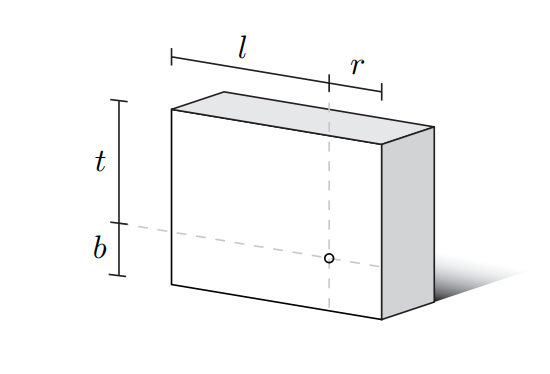
\includegraphics[width=0.7\textwidth]{figures/Preliminaries/off-axis.png}
    \caption{}\label{Off-axis projection}
\end{figure}

\clearpage